\chapter{Задача стабилизации с идеальным дифференцирующим звеном}
Рассмотрим объект управления 2-го порядка, заданный дифференциальным 
уравнением:
\[
a_2\ddot{y} + a_1\dot{y} + a_0y = u
\]

Возьмем $a_2 = 1$, $a_1 = -1$, $a_0 = 1$ для того, чтобы система имела хотя
бы один неустойчивый полюс. Получим уравнение:
\[
\ddot{y} - \dot{y} + y = u
\]

Зададим начальные условия:
\[
y(0) = 0, \quad \dot{y}(0) = 1
\]

Построим схему в Simulink и проведем моделирование:
\begin{figure}[H]
    \centering
    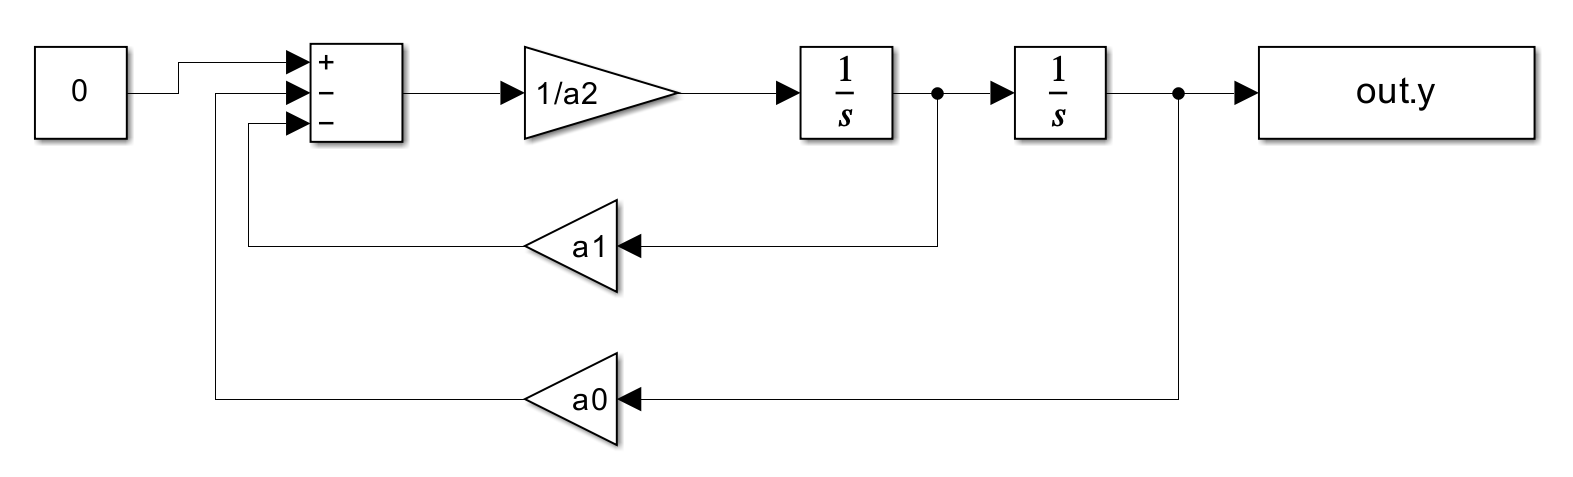
\includegraphics[width=1\textwidth, trim={0cm 0cm 0cm 0cm}]{../images/sim1.png}
    \caption{Схема разомкнутой системы в Simulink} 
\end{figure}
\begin{figure}[H]
    \centering
    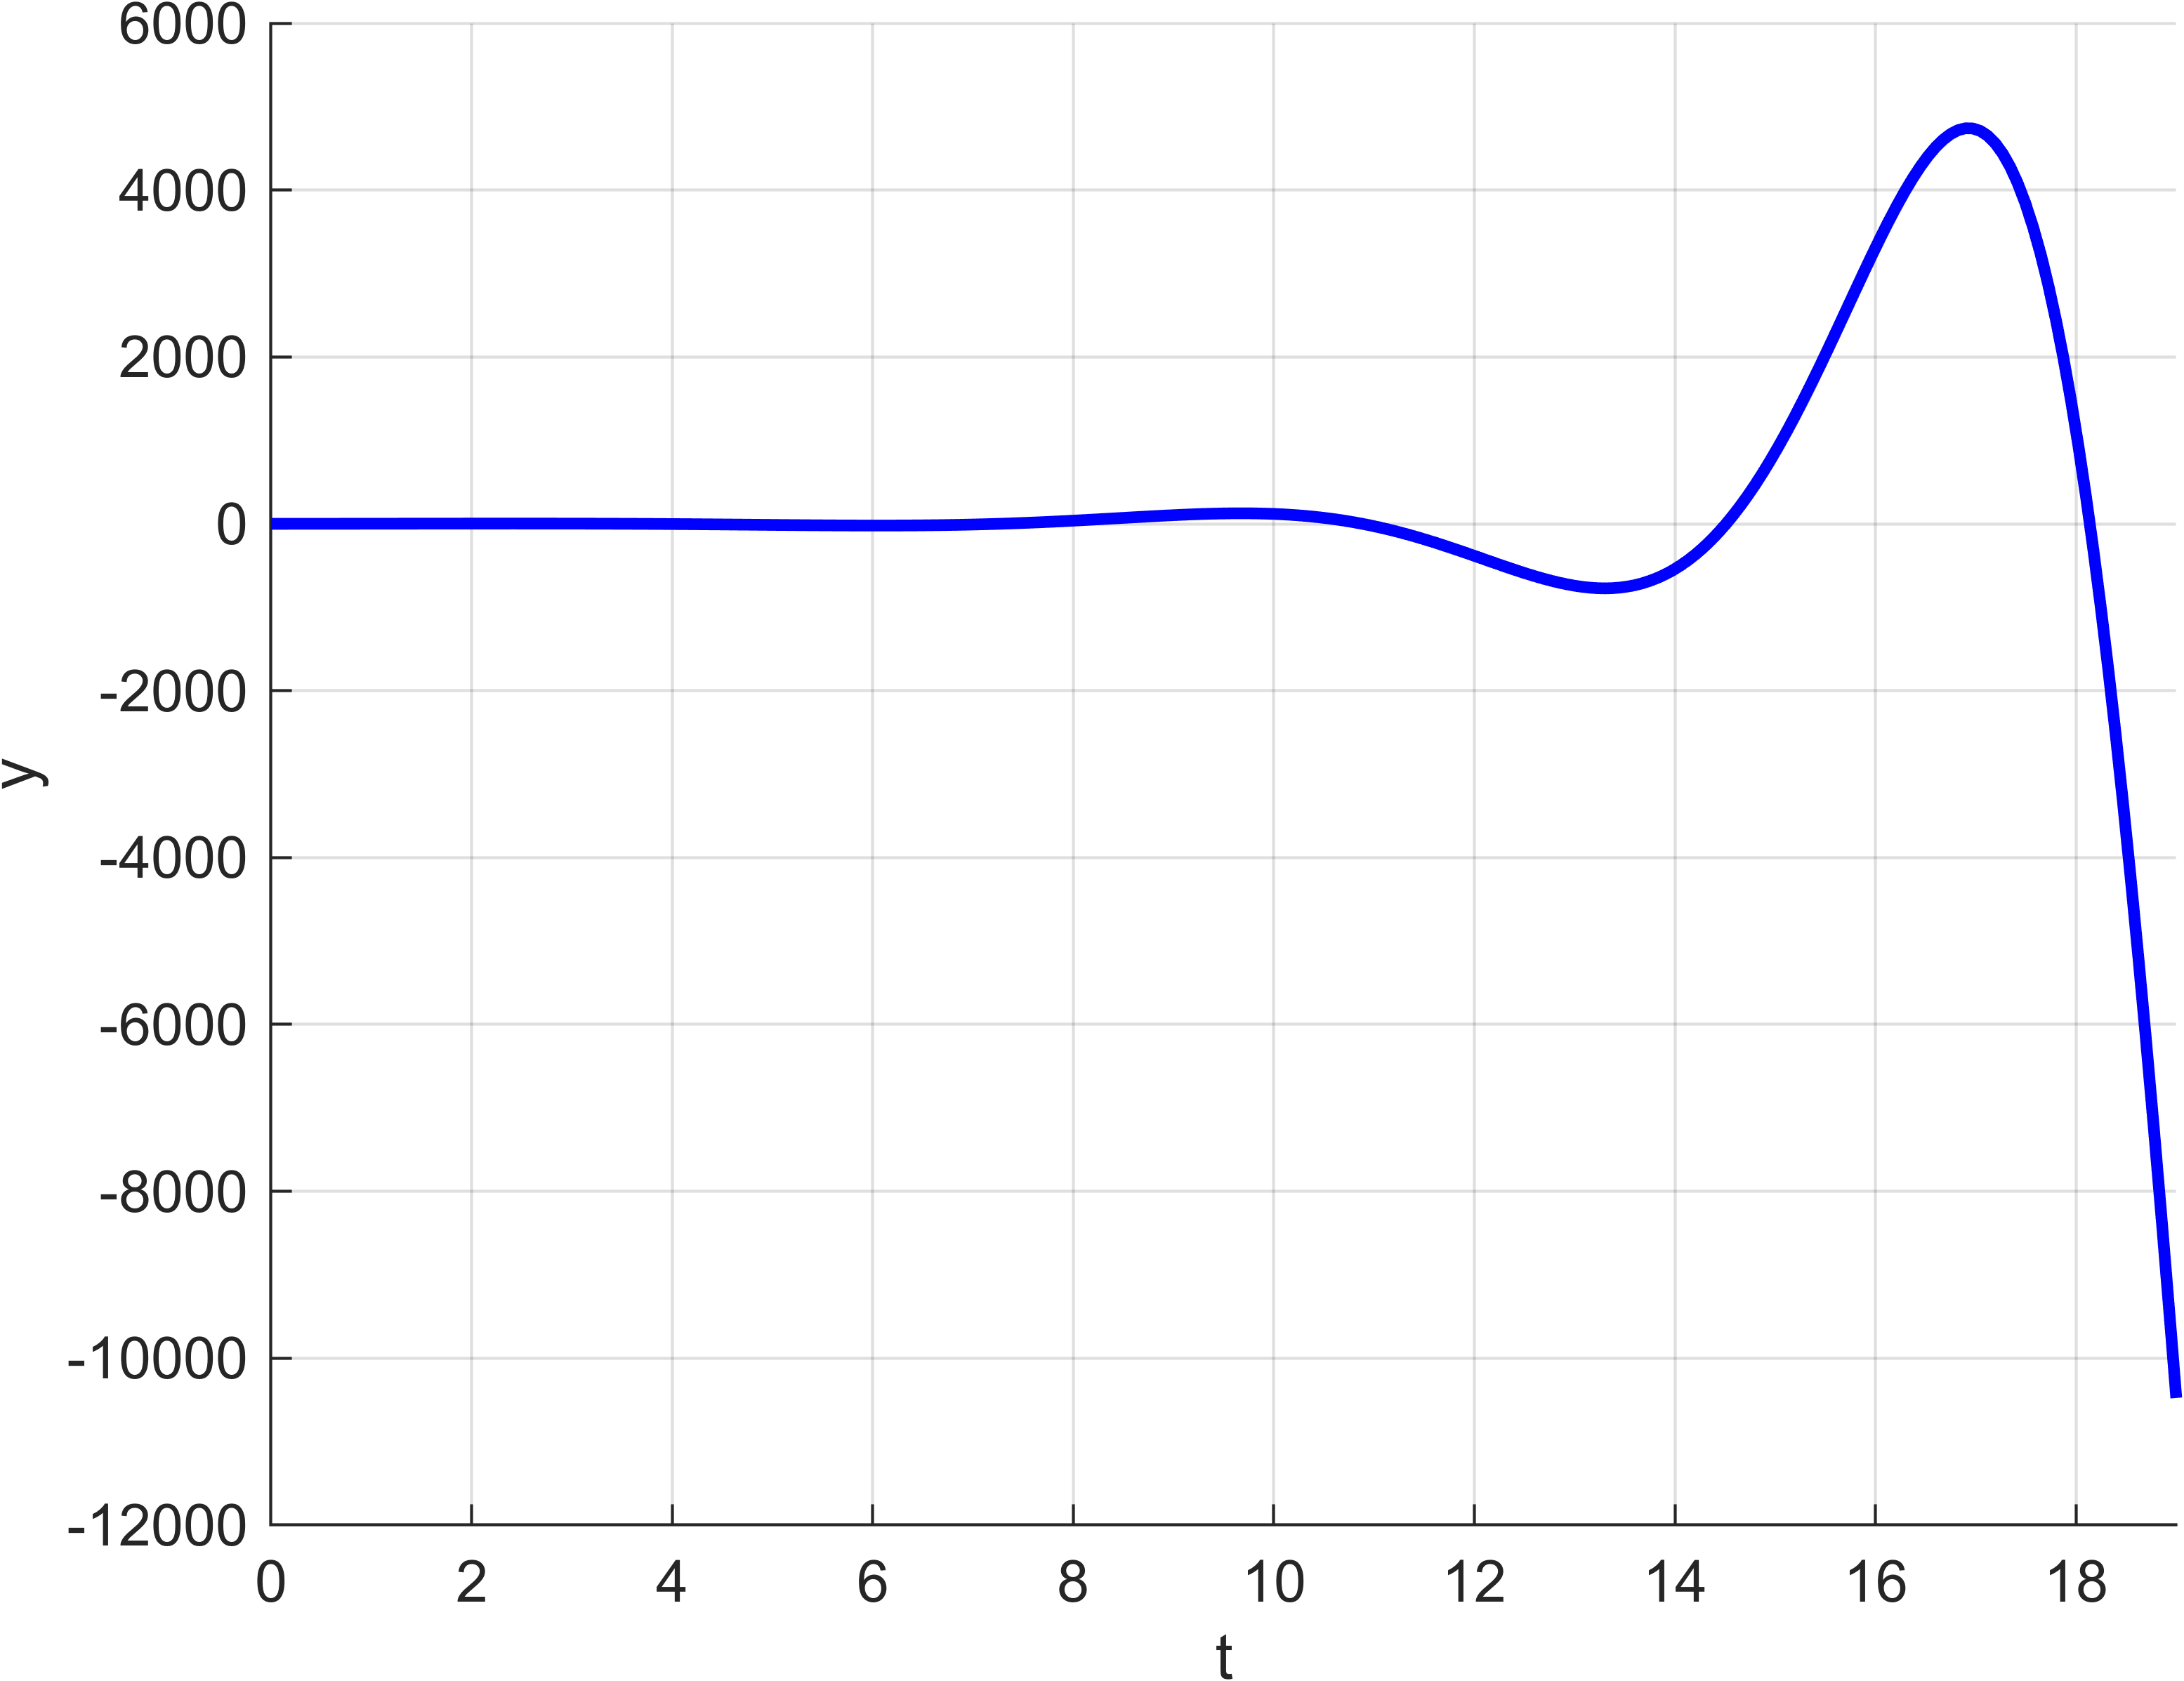
\includegraphics[width=1\textwidth, trim={0cm 0cm 0cm 0cm}]{../images/1_1.png}
    \caption{Сигнал разомкнутой системы $y_{\text{раз}}(t)$} 
\end{figure}

Рассмотрим регулятор вида:
\[
u = k_0y + k_1\dot{y}
\]

Построим структурную схему замкнутой системы, состоящей из объекта 
управления и регулятора, в режиме стабилизации:

\begin{figure}[H]
    \centering
    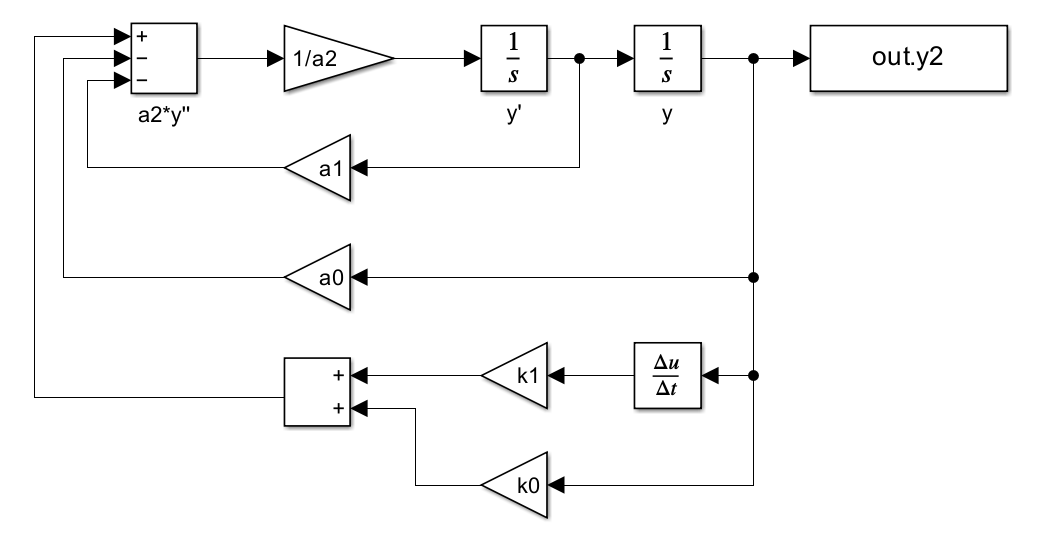
\includegraphics[width=1\textwidth, trim={0cm 0cm 0cm 0cm}]{../images/sim2.png}
    \caption{Схема замкнутой системы в Simulink}
\end{figure}

Найдем параметры $k_0$ и $k_1$, обеспечивающие асимптотически устойчивую замкнутую систему: 
\[
\ddot{y} - \dot{y} + y = k_0y + k_1\dot{y}
\]
\[
\ddot{y} + \dot{y}(-1 - k_1) + y(1 - k_0) = 0
\]
\[
\begin{cases}
    1 - k_0 > 0 \\
    -1 - k_1 > 0
\end{cases}
\]
\[
\begin{cases}
    k_0 < 1 \\
    k_1 < -1
\end{cases}
\]

Возьмем $k_0 = 1$, $k_1 = -3$ и проведем моделирование. А также сопоставим графики $y_{\text{раз}}(t)$ и $y_{\text{з}}(t)$:
\begin{figure}[H]
    \centering
    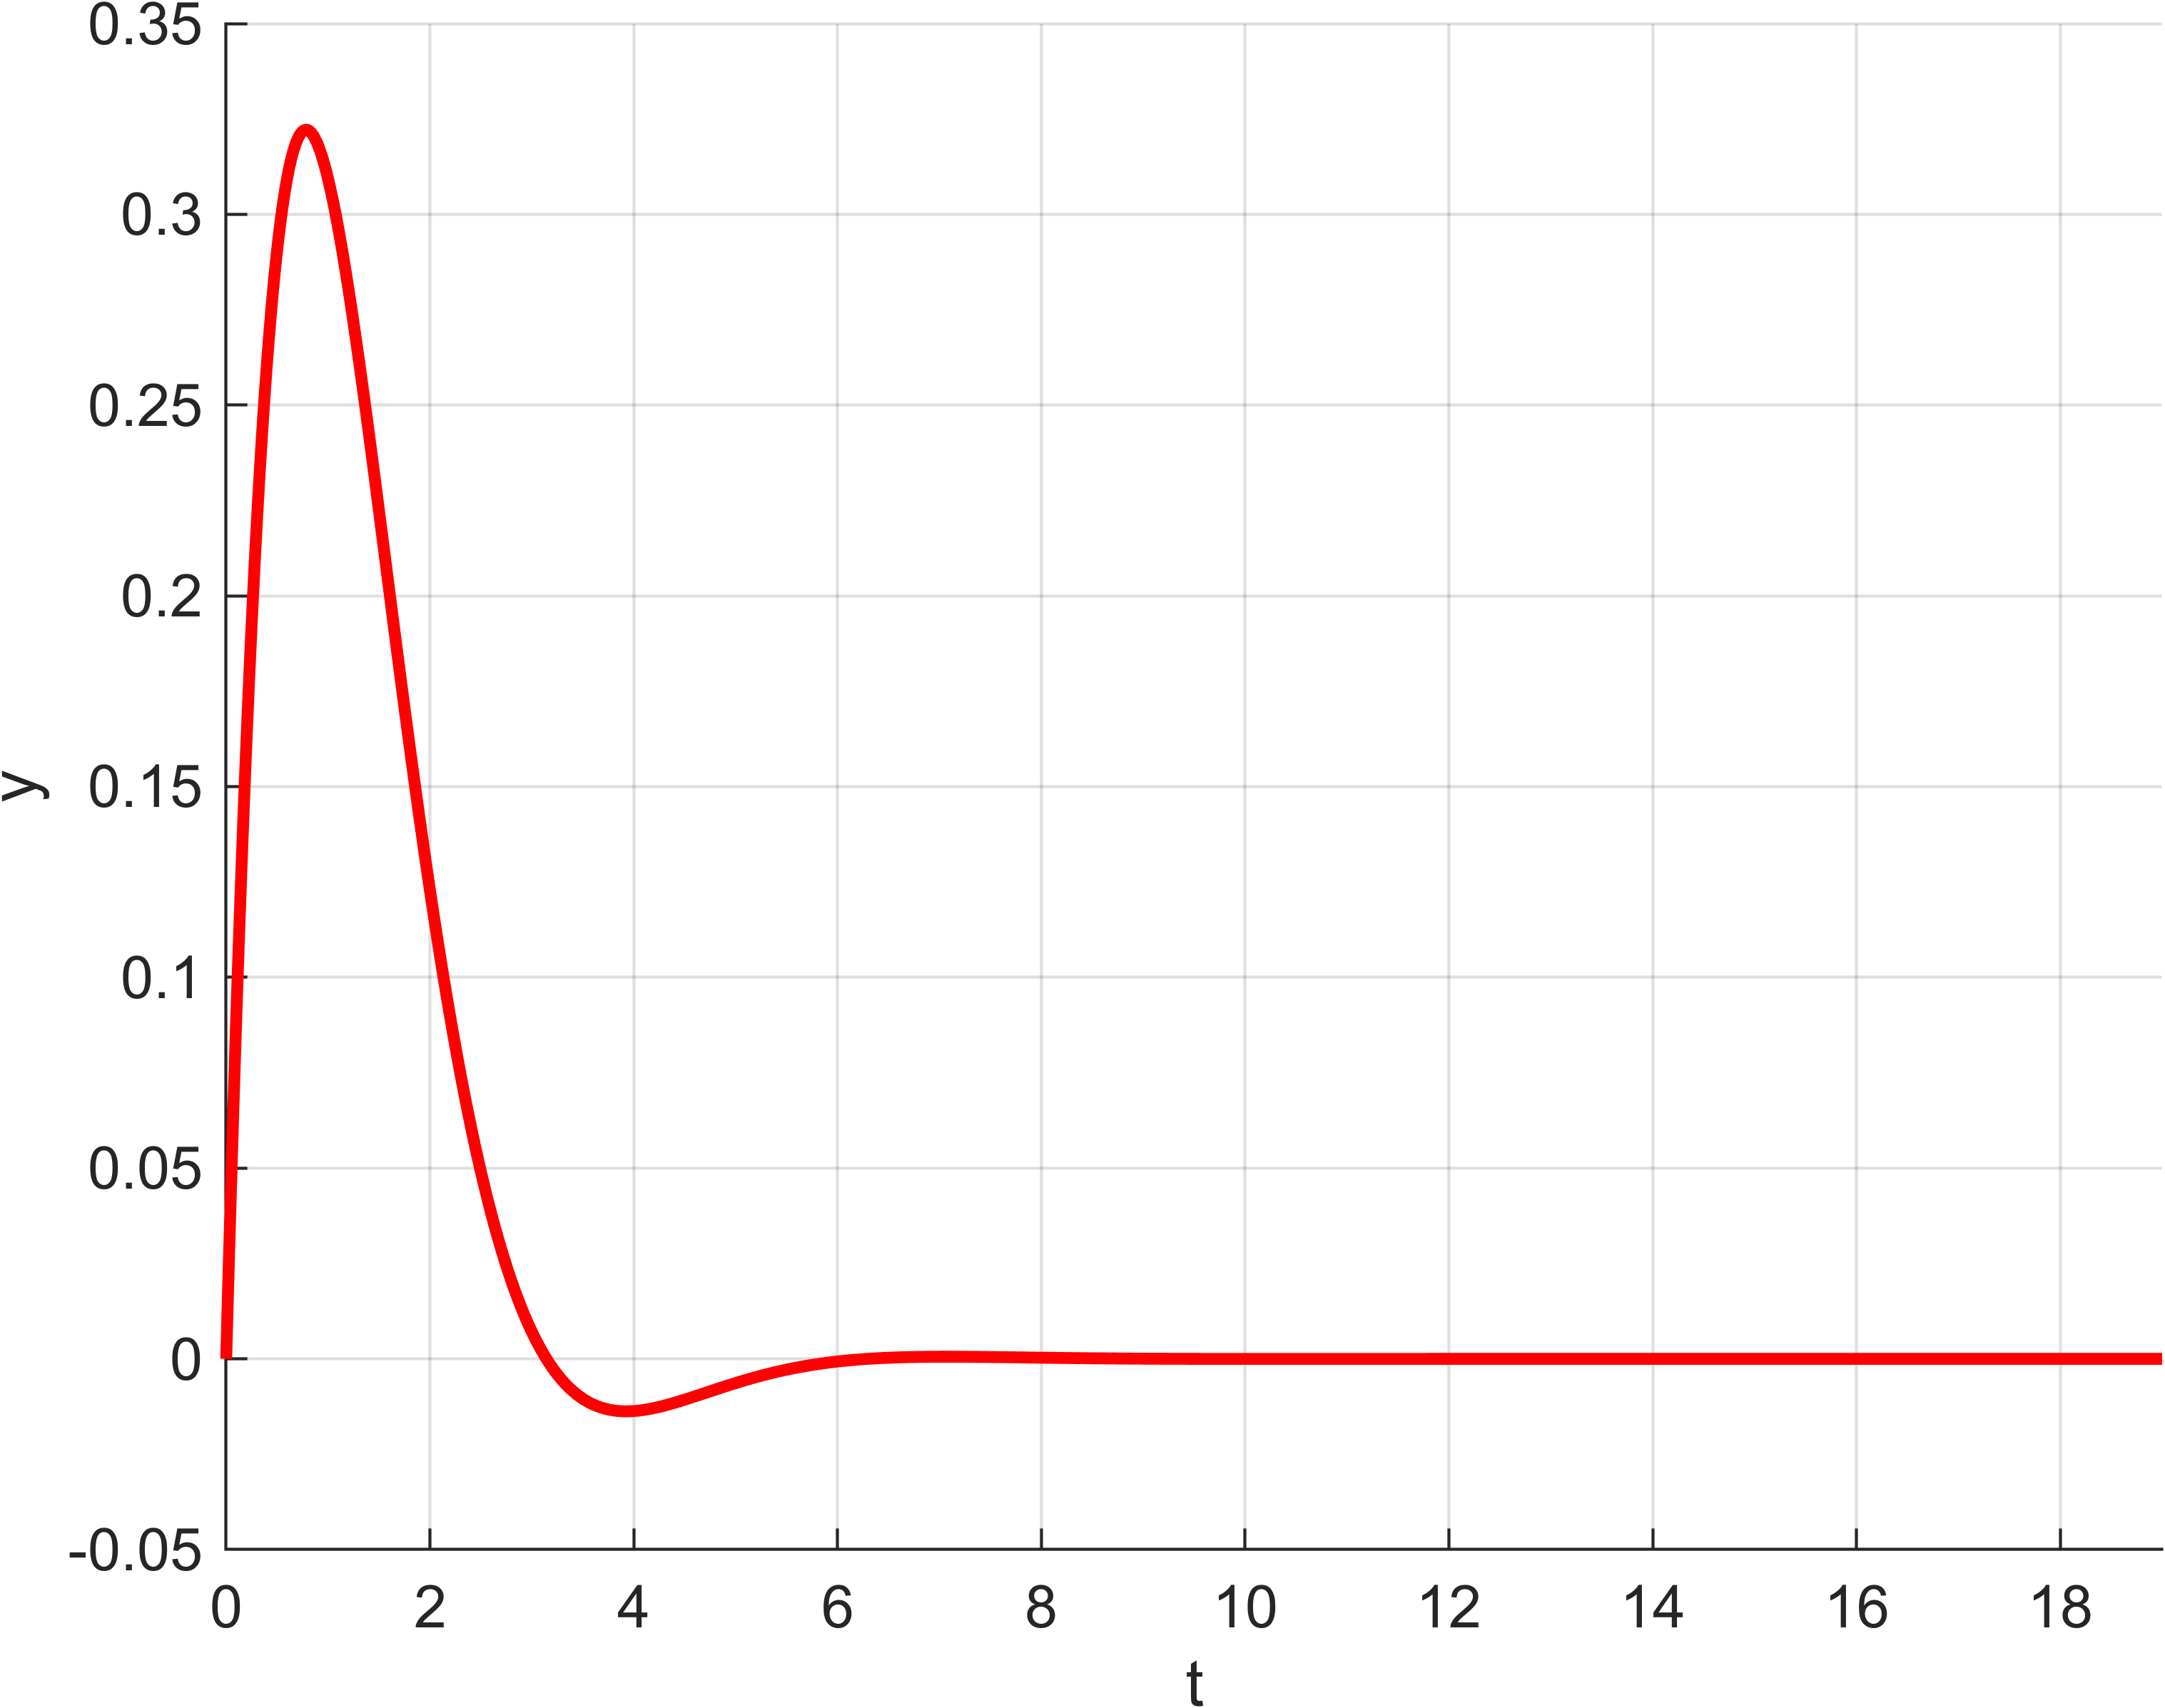
\includegraphics[width=0.75\textwidth, trim={0cm 0cm 0cm 0cm}]{../images/1_2.png}
    \caption{Сигнал замкнутой системы $y_{\text{з}}(t)$}
\end{figure}

\begin{figure}[H]
    \centering
    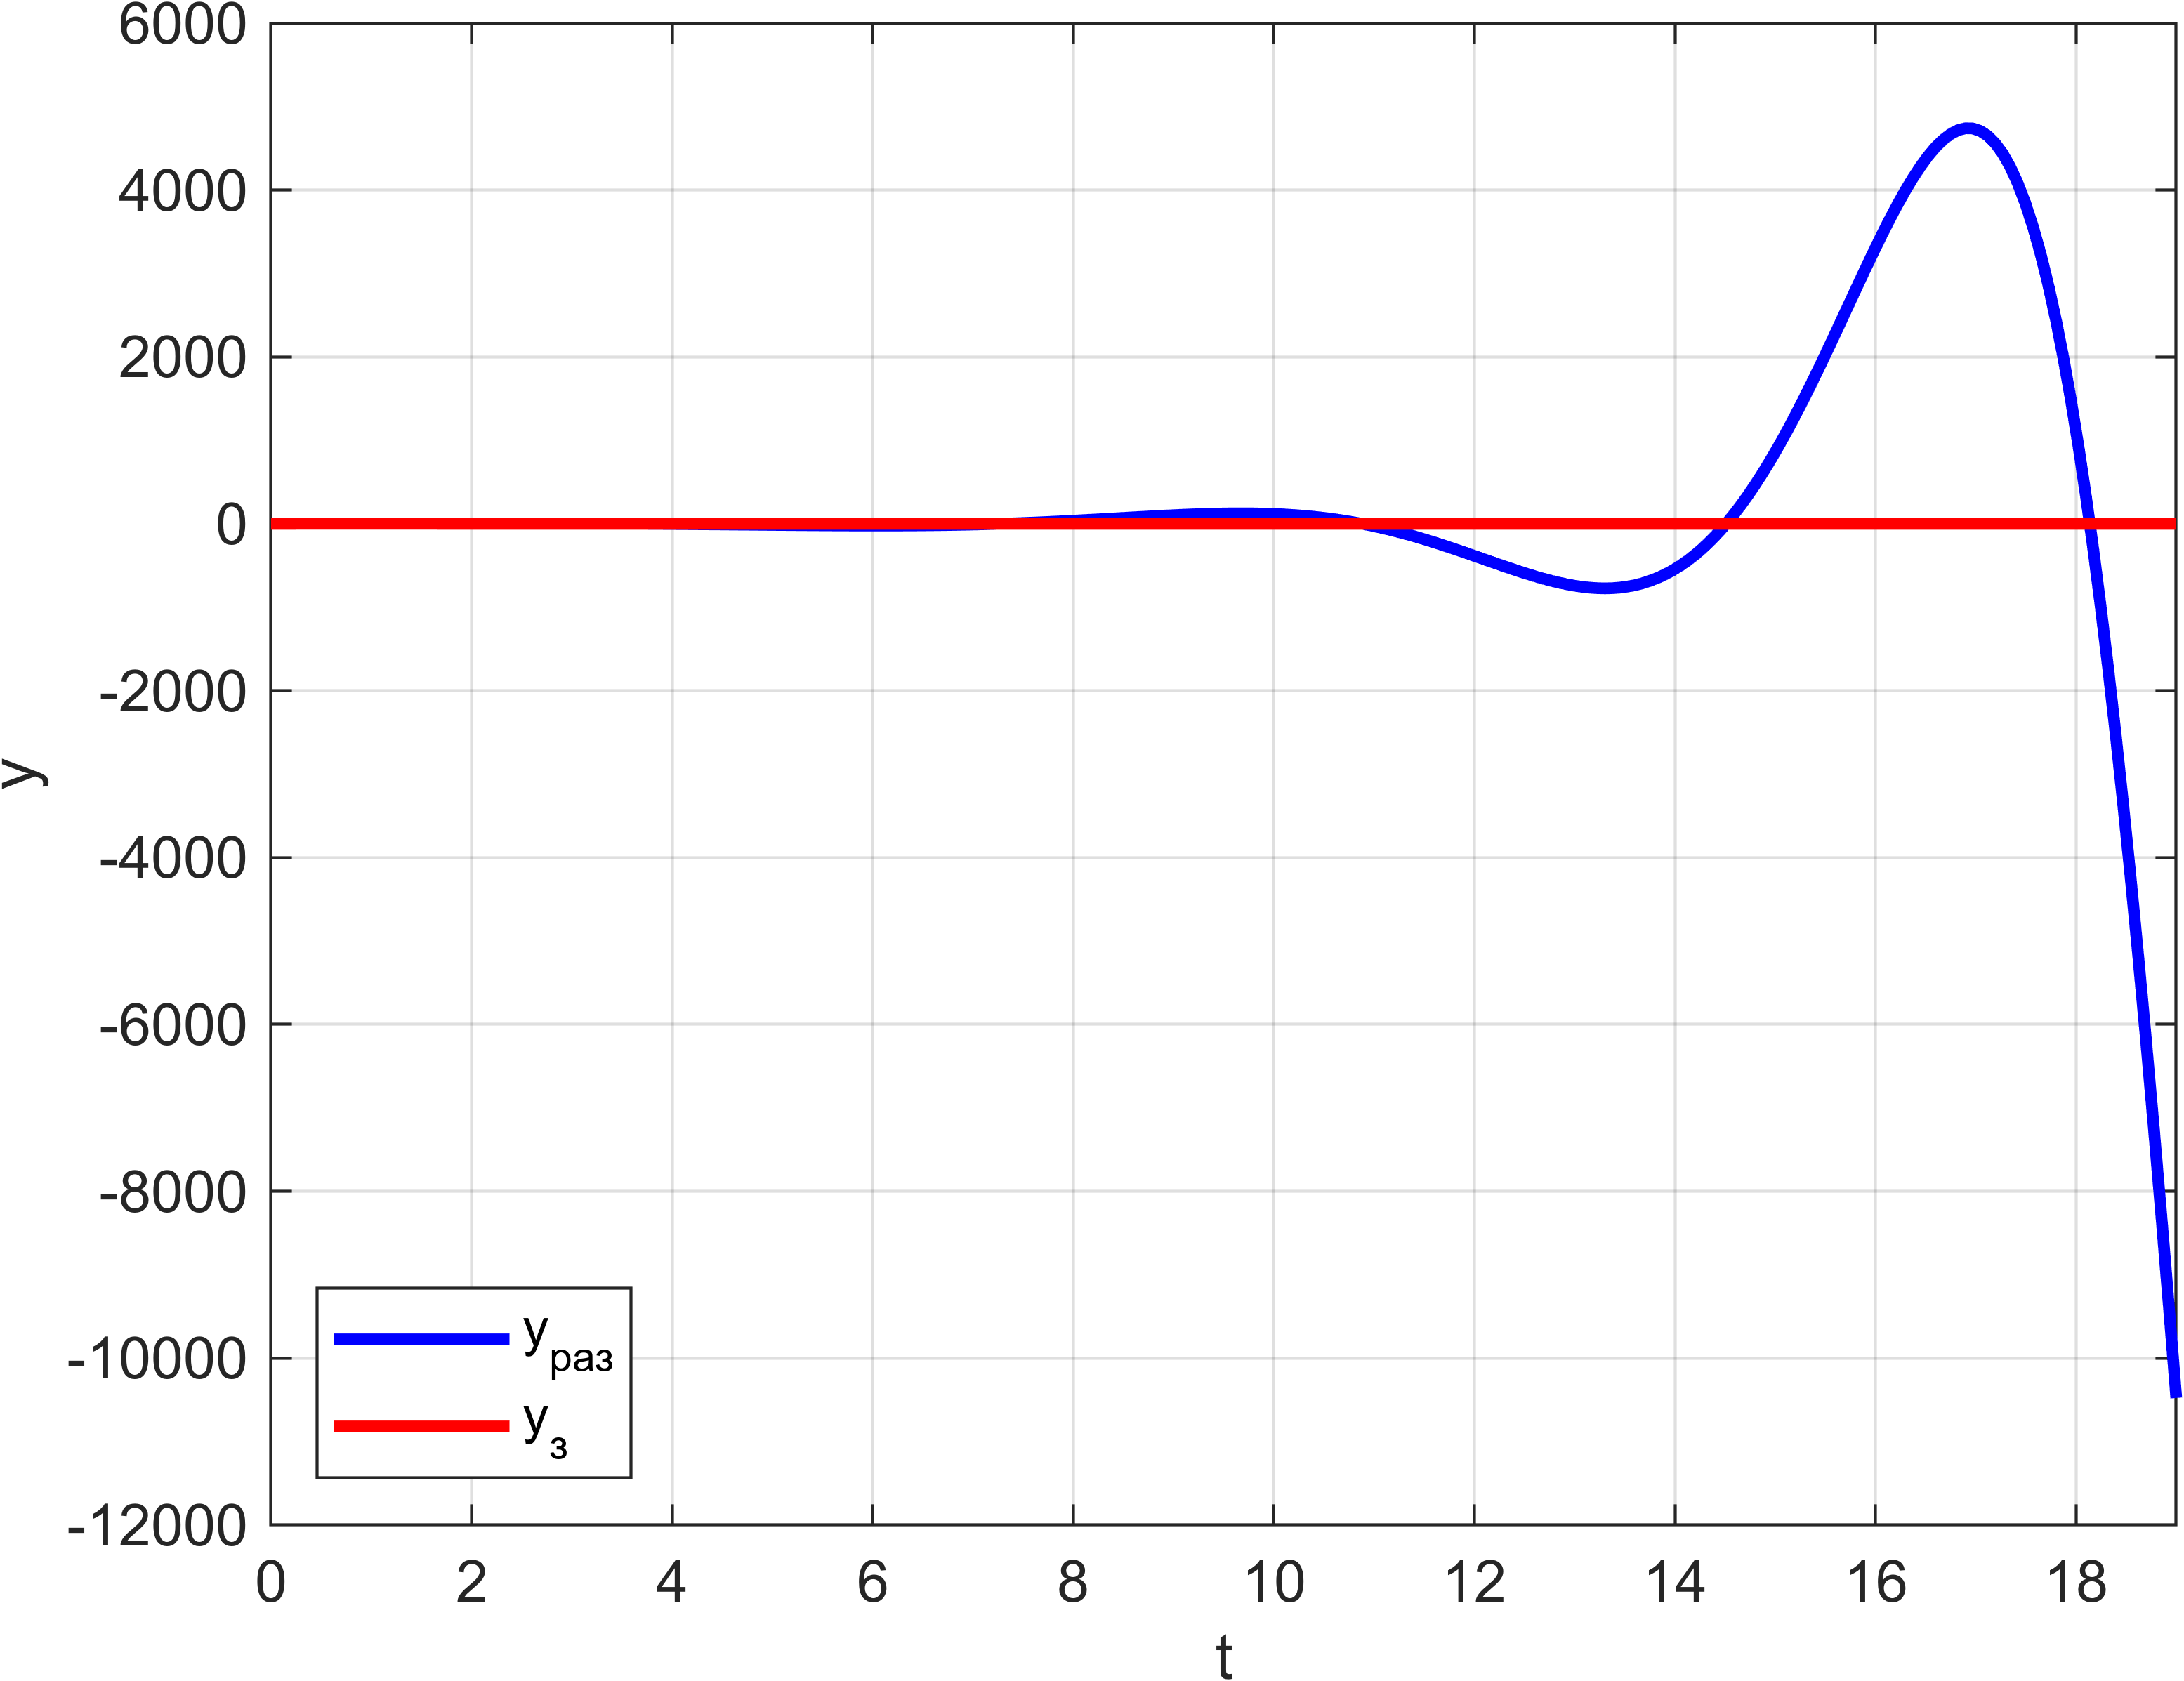
\includegraphics[width=0.75\textwidth, trim={0cm 0cm 0cm 0cm}]{../images/1_3.png}
    \caption{Сравнение сигналов $y_{\text{раз}}(t)$ и $y_{\text{з}}(t)$}
\end{figure}

Из графиков видно, что регулятор с идеальным дифференцирующим звеном
весьма хорошо обеспечивает стабилизацию системы.
\endinput